Last out is the ``friends'' test case. As there's a lot of data points for this case, the results have been split in two; one logarithmic view giving a rough overview of how the nodes performed (\autoref{fig:friends-log}), and one cropped view, where only edges with latency less than 500ms is included (\autoref{fig:friends-lin}). As we can see from the linear chart, there's only four nodes that observe latencies below 500ms, and not even all of those can reasonably be expected to be able to hold a conversation. A and B can talk together; A and E can talk, although a little more strained with latencies around 400ms. B and E can not talk, as B doesn't receive E's stream in reasonable time; B and F however \emph{can} talk together.

To summarize, out of 42 pairs of nodes in the test case, only three of them are able to communicate bidirectionally. In practice, this is a conversation all parties abandon immediately, as it's useless.

\autoref{fig:friends-getstats-bitrates} shows that for resource-constrained nodes, those resources are not distributed evenly among its peers. We see this in the data for node G, which is constrained to 9/4 bandwidth. Of it's 4Mbps, we see that node E receives a little more than 1Mbps of this, while the two other nearby nodes (D and F) lie around 500kbps each. Among the remote nodes, node C receives $\approx$350kbps, while A and B share the scraps that remain, with $\approx$200kbps each.

We observe something similar for nodes C and D, which are constrained to 8Mbps and 9Mbps, respectively. Well, almost -- node C is well received by nodes B, D and E, while nodes A and F are left with hardly anything -- which shows that being local or remote \emph{does not} seem to significantly influence who gets a fair share. Granted, this dataset is only from one single test run, more data is needed to say anything conclusively about whether this is expected behavior, but our data seem to imply that even a minute is not enough to reach fairness for Chrome.

Node D repeats much of what we saw in node C, but with a stronger bias towards \emph{remote} nodes, which all got more than any individual local node. This might be due to D being the first of the second group into the conversation, establishing connections with the remote nodes before any of the other local nodes are present. Thus when the other nodes in D's group joins, they get to share whatever capacity D has left. How the distribution evolves with time was not studied in this thesis, but might provide insight into how long it would take to reach fairness.

In any case, if it takes more than 10-30 seconds to establish fairness, we consider it likely that the users will leave the platform and not wait for stuff to smoothen out, at least if video is of any importance in the conversation. Audio will not be hit as hard by uneven distribution, but if your goal as a service provider is to deliver video conferencing, video quality and quick connection times will be how you're compared to other providers.

Uneven uplink distribution is not only bad for fairness in the conversation, but also for battery consumption. We can assume node G's video is encoded at least three times, possibly four in this test case\footnote{A and B could have shared the same stream, C, D and F could have shared a stream, and E has a stream of its own}, even though all of the nodes have spare downlink capacity for sharing one $\approx$600kbps stream ($4\text{Mbit}/6$).


\begin{figure}
    \centering
    \begin{subfigure}[t]{\textwidth}
        \centering
        \begin{tikzpicture}
        \begin{axis}[
            ylabel=Bitrate (bps),
            bar width=3,
            height=240,
            symbolic x coords={A,B,C,D,E,F,G},
            enlargelimits=0.10
            ]
            \input{data/appear.in-friends/bitrate.tex}
        \end{axis}
        \end{tikzpicture}
        \subcaption{Firefox}
    \end{subfigure}
    \begin{subfigure}[t]{\textwidth}
        \centering
        \begin{tikzpicture}
        \begin{axis}[
            ylabel=Bitrate (bps),
            ymax=2500000,
            symbolic x coords={A,B,C,D,E,F,G},
            bar width=3,
            height=240,
            enlargelimits=0.10,
            ]
        \input{data/appear.in-final-friends/bitrate-getstats.tex}
        \end{axis}
        \end{tikzpicture}
        \subcaption{Chrome}
    \end{subfigure}
    \caption{Bitrates for test case ``friends''}
    \label{fig:friends-bitrate}
\end{figure}

\begin{figure}
    \centering
    \begin{tikzpicture}
    \begin{axis}[
        ymode=log,
        axis x line=bottom,
        ylabel=Latency (ms),
        symbolic x coords={A,B,C,D,E,F,G},
        bar width=3,
        height=240,
        enlargelimits=0.10,
        ]
        \input{data/appear.in-friends/latency.tex}
    \end{axis}
    \end{tikzpicture}
    \caption{Test results for the ``friends'' test case in Firefox, log scale}
    \label{fig:friends-latency-log}
\end{figure}

\begin{figure}
    \centering
    \begin{subfigure}{\textwidth}
        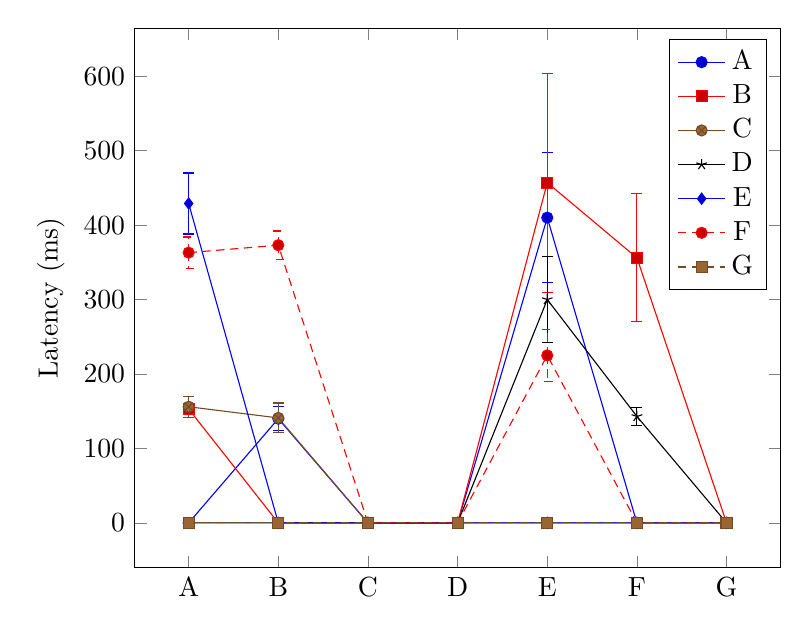
\begin{tikzpicture}
        \begin{axis}[
            ylabel=Latency (ms),
            symbolic x coords={A,B,C,D,E,F,G},
            bar width=3,
            height=240,
            enlargelimits=0.10,
            ]
            %% Traffic going out to A
\addplot+[error bars/.cd,y dir=both, y explicit]
coordinates{
    (A,0) +- (0.0, 0)
    (B,140) +- (0.0, 16)
    (C,0) +- (0.0, 0)
    (D,0) +- (0.0, 0)
    (E,410) +- (0.0, 87)
    (F,0) +- (0.0, 0)
    (G,0) +- (0.0, 0)
    };

%% Traffic going out to B
\addplot+[error bars/.cd,y dir=both, y explicit]
coordinates{
    (A,153) +- (0.0, 6)
    (B,0) +- (0.0, 0)
    (C,0) +- (0.0, 0)
    (D,0) +- (0.0, 0)
    (E,457) +- (0.0, 147)
    (F,356) +- (0.0, 86)
    (G,0) +- (0.0, 0)
    };

%% Traffic going out to C
\addplot+[error bars/.cd,y dir=both, y explicit]
coordinates{
    (A,156) +- (0.0, 14)
    (B,141) +- (0.0, 20)
    (C,0) +- (0.0, 0)
    (D,0) +- (0.0, 0)
    (E,0) +- (0.0, 0)
    (F,0) +- (0.0, 0)
    (G,0) +- (0.0, 0)
    };

%% Traffic going out to D
\addplot+[error bars/.cd,y dir=both, y explicit]
coordinates{
    (A,0) +- (0.0, 0)
    (B,0) +- (0.0, 0)
    (C,0) +- (0.0, 0)
    (D,0) +- (0.0, 0)
    (E,300) +- (0.0, 58)
    (F,143) +- (0.0, 12)
    (G,0) +- (0.0, 0)
    };

%% Traffic going out to E
\addplot+[error bars/.cd,y dir=both, y explicit]
coordinates{
    (A,429) +- (0.0, 41)
    (B,0) +- (0.0, 0)
    (C,0) +- (0.0, 0)
    (D,0) +- (0.0, 0)
    (E,0) +- (0.0, 0)
    (F,0) +- (0.0, 0)
    (G,0) +- (0.0, 0)
    };

%% Traffic going out to F
\addplot+[error bars/.cd,y dir=both, y explicit]
coordinates{
    (A,363) +- (0.0, 21)
    (B,373) +- (0.0, 19)
    (C,0) +- (0.0, 0)
    (D,0) +- (0.0, 0)
    (E,225) +- (0.0, 35)
    (F,0) +- (0.0, 0)
    (G,0) +- (0.0, 0)
    };

%% Traffic going out to G
\addplot+[error bars/.cd,y dir=both, y explicit]
coordinates{
    (A,0) +- (0.0, 0)
    (B,0) +- (0.0, 0)
    (C,0) +- (0.0, 0)
    (D,0) +- (0.0, 0)
    (E,0) +- (0.0, 0)
    (F,0) +- (0.0, 0)
    (G,0) +- (0.0, 0)
    };

\legend{A, B, C, D, E, F, G}

        \end{axis}
        \end{tikzpicture}
        \subcaption{Firefox, only sub-500ms values}
    \end{subfigure}
    \begin{subfigure}[t]{\textwidth}
        \centering
        \begin{tikzpicture}
        \begin{axis}[
            ymax=600,
            ylabel=Latency (ms),
            symbolic x coords={A,B,C,D,E,F,G},
            bar width=3,
            height=240,
            enlargelimits=0.10,
            ]
            \input{data/appear.in-final-friends/latency-getstats.tex}
        \end{axis}
        \end{tikzpicture}
        \subcaption{Chrome}
    \end{subfigure}
        \caption{Observed latencies in the ``friends'' test case}
    \label{fig:friends-latency}
\end{figure}
